\section{Эксперемент}
\subsection{Часть}
\begin{equation} 
    K2Cr2O7 + 14HCl \xrightarrow{}  2KCl + 2CrCl3 + 7H2O + 3Cl2
\end{equation} 
\begin{figure}[h]
    \centering
    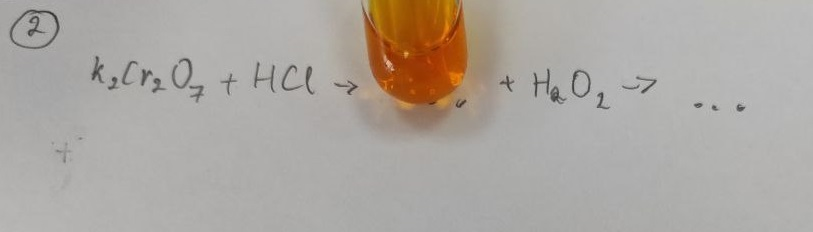
\includegraphics[width=1\linewidth]{Ex_3/Ex_3_1_1.jpg}
     \caption{}
    \label{ex_3_1_1}
\end{figure}
\begin{equation} 
    2KCl + 2CrCl_3 + 7H_2O + 3Cl_2 
    \xrightarrow{} 2KCl + 2CrCl_ 4 + 8H_2O 
\end{equation} 
\begin{figure}[h]
    \centering
    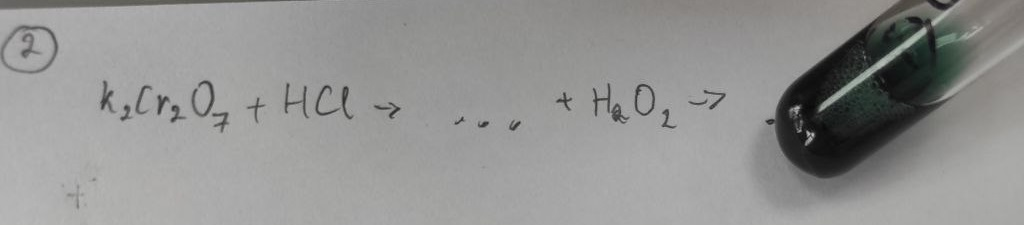
\includegraphics[width=1\linewidth]{Ex_3/Ex_3_1_2.jpg}
     \caption{}
    \label{ex_3_1_2}
\end{figure}


\subsection{Часть}
\begin{equation} 
    2KMnO_4 + 16HCl \xrightarrow{} 
    2KCl + 2MnCl_2 + 5Cl_2 + 8H_2O
\end{equation} 
\begin{figure}[h]
    \centering
    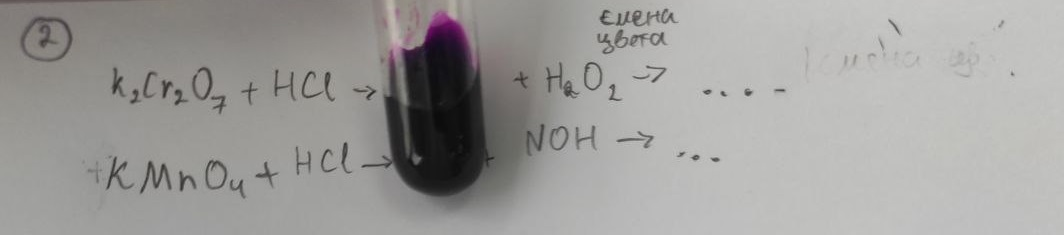
\includegraphics[width=1\linewidth]{Ex_3/Ex_3_2_1.jpg}
     \caption{}
    \label{ex_3_2_1}
\end{figure}
\begin{equation} 
    2KMnO_4 + 3Na_2SO_3 + 4H_2SO_4 \xrightarrow{}\, 
    K_2SO_4 + 2MnSO_4 + 3Na_2SO_4 + 4H_2O 
\end{equation} 

\begin{figure}[h]
    \centering
    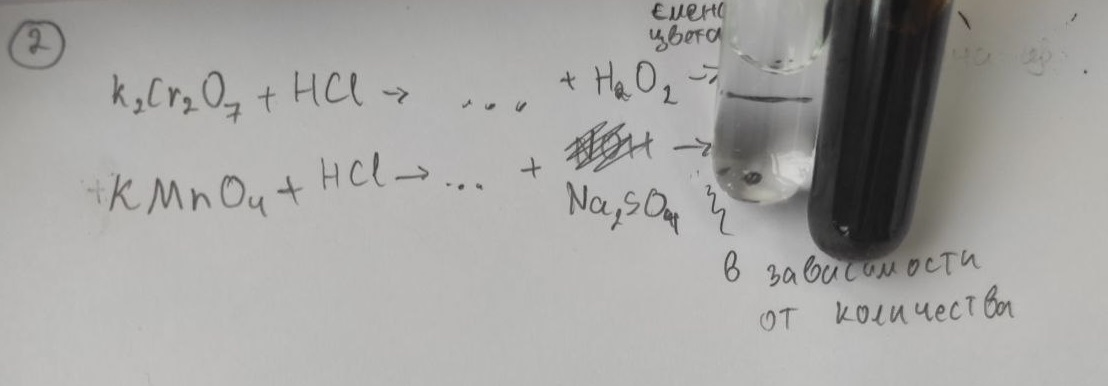
\includegraphics[width=1\linewidth]{Ex_3/Ex_3_2_2.jpg}
     \caption{Если добавить немного серной кислоты цвет темно коричневый но при дальнейшем доабавлении цвет терятся}
    \label{ex_3_2_2}
\end{figure}

\begin{eqnarray} 
    2KMnO_4 + 3Na_2SO_4 + 2NaOH &\xrightarrow{}& 
    2MnO_2 + 3Na_2SO_4 + 2KOH + 2NaNO_3\\
    2MnO4^- + 5SO_4^{2-} + 16H^+ + 2Na^+ + 2OH^- &\xrightarrow{}& 
    2MnO_2 + 3Na^+ + 3SO4^{2-} + 2K^+ + 2OH^- + 2Na^+ + 2NO_3^-
\end{eqnarray} 